
\documentclass[times, 12pt,twocolumn]{article} 
\usepackage{latex8}
\usepackage{times}
\usepackage[ngerman]{babel}
\usepackage{todonotes}
\usepackage[utf8]{inputenc}
\usepackage{graphicx}
\usepackage[hyphens]{url}
\usepackage{mathtools}
\usepackage{amsmath}
\usepackage{amssymb}
\usepackage[font=small,labelfont=bf]{caption}

\pagestyle{empty}


\begin{document}

\title{Neuronale Netze in der Videoproduktion}

\author{Laura Anger\\
Technische Hochschule K\"oln \\ Institut f\"ur Medien- und Phototechnik \\  laura.anger@th-koeln.de \\
\and
Vera Brockmeyer\\
Technische Hochschule K\"oln \\ Institut f\"ur Medien- und Phototechnik \\ vera.brockmeyer@smail.th-koeln.de \\
}

\maketitle
\thispagestyle{empty}


\large{\textbf{Zusammenfassung}}\\ \small %\normalsize
\todo[inline, color=red]{Vera} 

\large{\textbf{Schl\"usselw\"orter}}\\ \small %\normalsize
 Faltungsnetze, Videoproduktion
 \todo[inline, color=red]{Vera} 


\Section{Einleitung} \label{sec:Einleitung}
\todo[inline, color=yellow]{Vera} 
Die Videoproduktion konnte sich im Zuge der Digitalisierung im letzten Jahrzehnt enorm qualitativ verbessern. Jeder der vier Produktionabschnitte (siehe Abbildung~\ref{fig:Videoproduktion}) konnte verbessert und vor allem erleichtert werden. In der Konzeptionsphase konnten die Arbeitsprozesse mit Hilfe des Internets erleichtert werden durch den beschleunigten weltweiten Austausch von Skripten oder den standort-unabhängigen Zugriff auf cloudbasierte Projektmanagement Systeme.

Während der Produktion des Videomaterials unterstützen moderne digitale Kamerasysteme den Kameramann indem sie den Weißabgleich und die Belichtung automatisch berechnen und einstellen. Selbst geringfügige unruhige Bewegungen werden mit Bildstabilisatoren direkt unterdrückt. 

Die darauffolgenden Arbeitsprozesse, wie das Schneiden und Editieren des Videomaterials währen der Postproduktionsphase, wurden in den letzten Jahren vereinfacht oder können teilweise durch zuverlässige Algorithmen automatisch durchgeführt werden. Mittlerweile können realistisch virtuelle Bildinhalte von CGI Experten mit entsprechender Rechenkapazität in das gedrehte Videomaterial nahtlos rendert werden. Dies ermöglicht es Produktionen fast ausschließlich im Studio zu produzieren und sogar aufwendige Fantasywelten oder aufwendige Stunts mit geringeren Kosten umzusetzen.

Doch gerade qualitativ hochwertige Videoproduktionen erfordern immer noch einen sehr hohen Arbeitsaufwand mit einer große Anzahl an professionellen Mitarbeitern und teuren Materialien. Einen großen Anteil daran hat die Postproduktion in der jede Szene separat editiert und an das Gesamtbild angepasst werden muss. Dieses Gesamtbild muss vorab genau festgelegt werden, denn eine spätere Korrektur erfordert eine vollständige Wiederholung der meisten Arbeitsschritte. Aber auch die Generierung von Bildmaterialien für kurze Schnittszenen oder Webvideos ist sehr zeitaufwändig und teuer. Ein mehrköpfiges Team mit dem umfangreichen Equipment muss zum Drehort gebracht werden. 

In der Zukunft gilt es diesen Arbeits- und Kostenaufwand weiter zu reduzieren indem die einzelnen Arbeitsschritte automatisiert oder teil-automatisiert werden. Dies erfordert Ansätze die komplexe Zusammenhänge und Erfahrungen wie das menschliche Gehirn vereinen können. Sie sollten im idealen Fall Kreativität umsetzen, Bewegungen und Abläufe voraussagen, bekannte Eigenschaften sinnvoll kombinieren oder erlernte Informationen übertragen und anwenden können. Diese Anforderungen können mit einer Form von künstlichen Intelligenz, den neuronalen Netzen (NN) (siehe Abschnitt~\ref{sec:Faltungsnetze}), erfolgreich erfüllt werden, die jenen des menschlichen Gehirn nachempfunden sind. In den letzten Jahren wurden NN stetig weiterentwickelt und es konnten vor allem im Bereich der Medienproduktion bahnbrechende Erfolge erzielt werden. Die vielversprechendsten Erfolge konnten mit einer besonderen Form der NN erzielt werden. Diese Faltungsnetze (CNN) (siehe Abschnitt~\ref{sec:Faltungsnetze}) ermöglichen orts- und skalierungs-unabhängige Operationen und somit ideal für mehrdimensionale digitale Signale.\\

Zu Beginn wurden CNN zur Objektklassifizierung eingesetzt um unter anderem automatisch Metadaten von Bild- oder Videodaten zu generieren und in Datenbanken oder Suchmaschinen einzupflegen. Ein bekannter Ansatz ist \textit{Clarifai}~\cite{MITReview}, welcher eine Bibliothek mit konfigurierten CNN anbietet um optimierte Datenbanken anzulegen und zu verwalten. In den letzten Jahren wurden sie auch verstärkt für die Generierung oder Fortsetzung von bekannten Daten oder Signalen eingesetzt. Es konnten klassische Musikstücke sinnvoll beliebig verlängert werden~\cite{OordDZSVGKSK16} oder bewegte Sequenzen aus einzelnen Bildern generiert werden~\cite{VondrickPT16}. Auch in der Postproduktion konnten neue Bilder erstellt werden~\cite{DeepDream}. \\

In den folgenden Kapiteln wird in den Grundlagen (siehe Kapitel~\ref{sec:Grundlagen}) auf den allgemeine Ablauf in der Videoproduktion sowie detailliert die Funktionsweise der NN und CNN beschrieben. Im Anschluss werden in den folgenden Kapiteln verschiedene Entwicklungen von Videoproduktionsmittel vorgestellt, welche verschiedene Formen von NN und im besonderen von CNN nutzen. Drei Ansätze werden detailliert beschrieben und bewertet. Der erste Ansatz~\cite{VondrickPT16} beschreibt in Anschnitt~\ref{sec:Vondrick} die Generierung von eine bewegten Bildsequenz aus einem Einzelbild. Die anderen Ansätze~ \cite{DeepDream}~\cite{GatysEB15a} erläutert die Übertragung eines Bildstils auf eine andere Videosequenz.


\Section {Grundlagen} \label{sec:Grundlagen}
\todo[inline, color=yellow]{Laura} 
Um gezielter Ansatzpunkte für den Einsatz von NNs in der Videoproduktion aufzeigen zu können, wird diese in Kapitel~\ref{sec:Videoproduktion} kurz beschrieben. Der Schwerpunkt dieses Kapitels liegt jedoch auf den Grundlagen von NNs und insbesondere CNNs, sowie deren Training.

\SubSection{Videoproduktion} \label{sec:Videoproduktion}
\todo[inline, color=yellow]{Laura} 
\begin{figure}
	\flushleft
	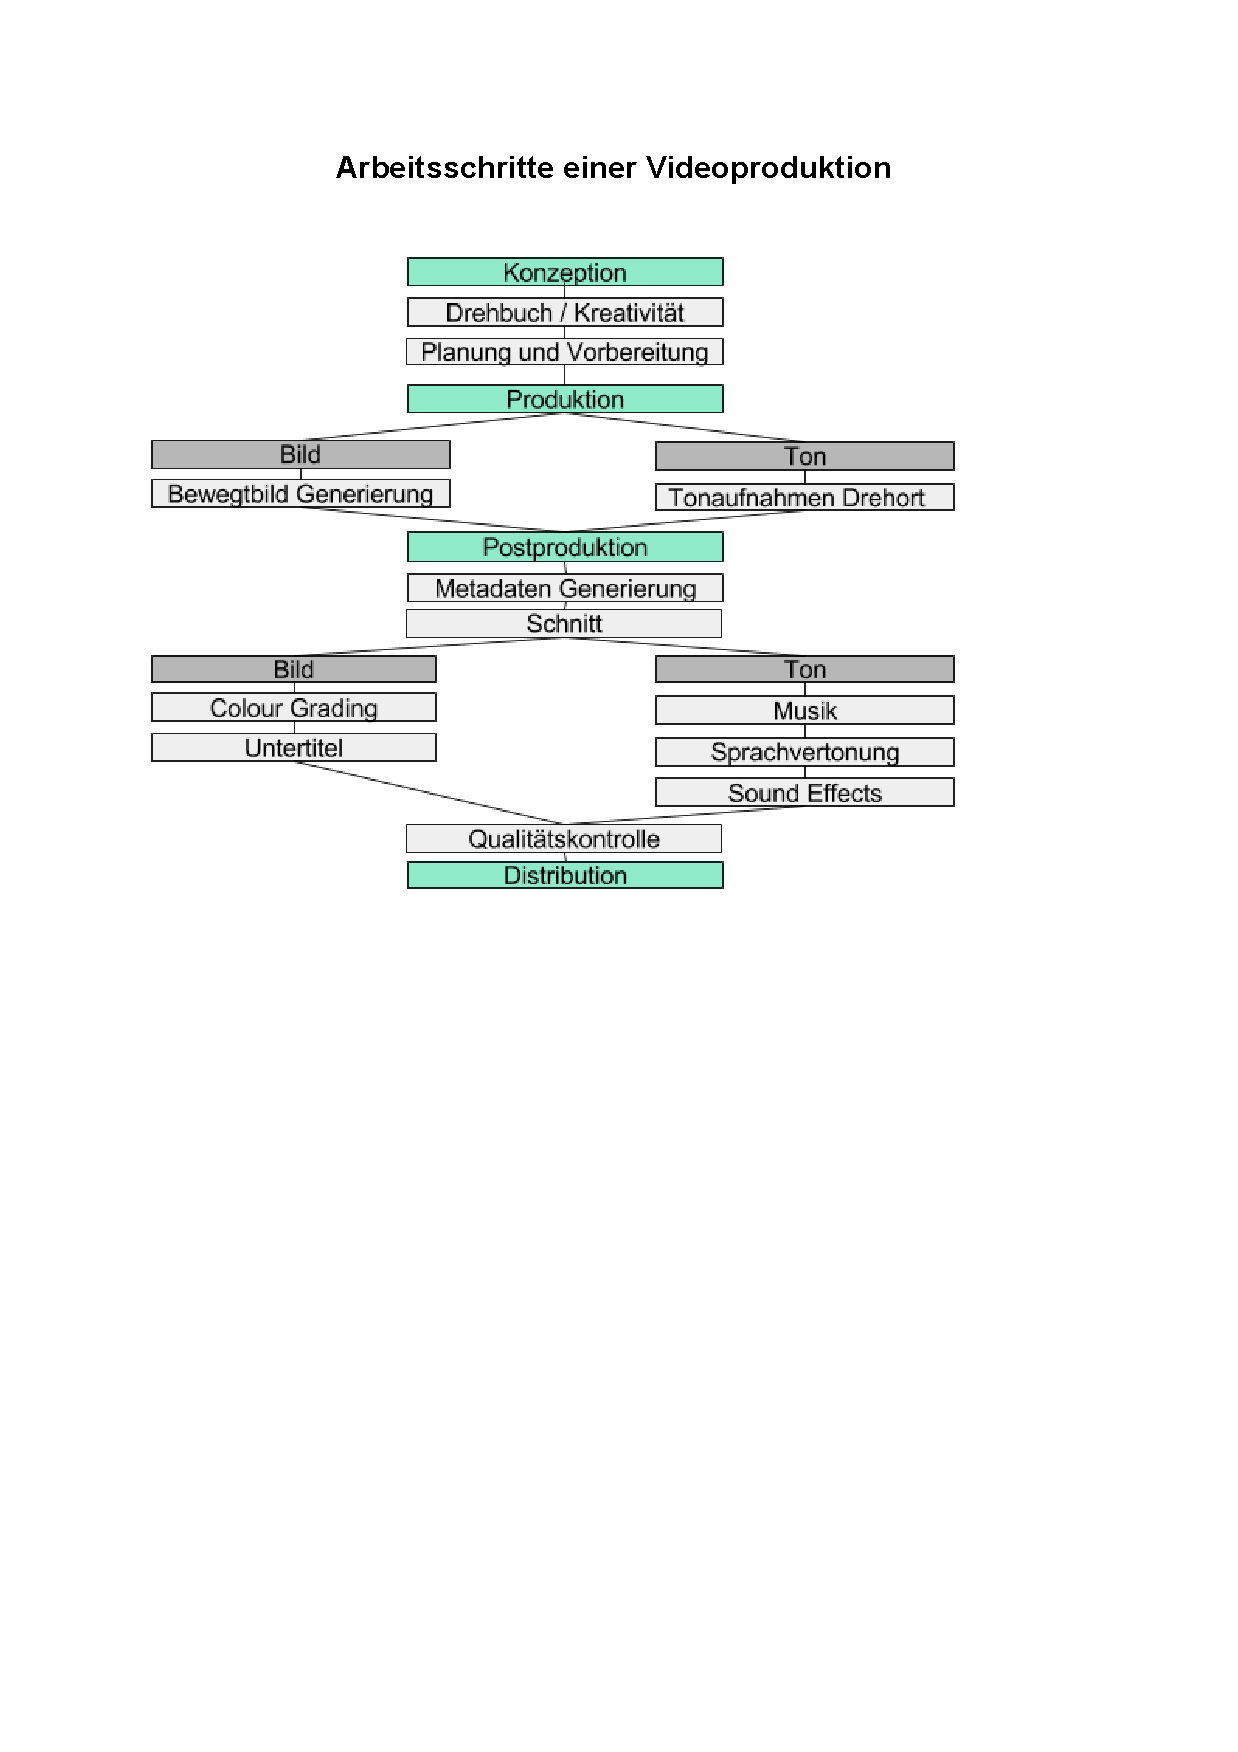
\includegraphics[width=\columnwidth, trim = 20mm 145mm 45mm 40mm, clip]{Bilder/ArbeitsschritteVideoproduktion.pdf}
	\caption{Grundlegende Arbeitsschritte einer Videoproduktion.}
	\label{fig:Videoproduktion}
\end{figure}
Mit der Videoproduktion oder auch Filmproduktion wird die Herstellung sowohl von Kino- als auch von Werbe- und Fernsehfilmen zusammengefasst. In Abbildung~\ref{fig:Videoproduktion} ist ein Ablaufplan einer typischen Videoproduktion zu sehen. Da es alleine in Deutschland über 850 Produktionsformen gibt (Stand 2014)~\cite{formatt}, kann der Ablaufplan nur einen sehr allgemeinen Überblick über die notwendigen Arbeitsschritte bieten. \\
Der erste Schritt, die Konzeption soll sowohl die Projektentwicklung, als auch die Vorproduktion zusammenfassen. Die sich anschließende Produktionsphase kann grob, wie im Schaubild zu sehen in Bild und Ton unterteilt werden, wobei diese beiden Bereiche nicht immer getrennt voneinander betrachtet werden sollten. Die Postproduktion besteht aus vielen verschiedenen Arbeitsschritten, deren Schwerpunkt auf dem Schnitt und der digitalen Bildnachbearbeitung liegt. Der Schritt der Distribution ist hier der Vollständigkeit halber erwähnt und beschreibt die Filmverwertung. \\
Der Aufbau der folgenden Ausführungen orientiert sich an Abbildung~\ref{fig:Videoproduktion} (vgl. Kapitel~\ref{sec:Konzeption},~\ref{sec:Produktion} und~\ref{sec:Postroduktion}).



\SubSection{Neuronale Netze} \label{sec:NeuronaleNetze}
\todo[inline, color=yellow]{Laura} 
NNs finden unter anderem Anwendung bei der Steuerung von Robotern, Börsenkursanalysen, Medizin oder Fahrzeugsteuerung. In der Bildverarbeitung werden NNs vor allem zur Klassifizierung genutzt. \\
Sie sind vom menschlichen Gehirn inspiriert, welches laut~\cite{NNHaykin} ein nicht-lineares, komplexes und hoch paralleles System zur Verarbeitung von Informationen darstellt. Ähnlich wie dieses bestehen künstliche NNs aus einer Menge an simulierten Neuronen, die untereinander verbunden sind und in Schichten organisiert sind. Es gibt verschiedene Arten der Vernetzung, die, wie in \cite{NNHaykin} und \cite{NNStanley} beschrieben, in rück- und vorwärts gekoppelte Modelle unterteilt werden können.\\
\begin{figure}
	\flushleft
	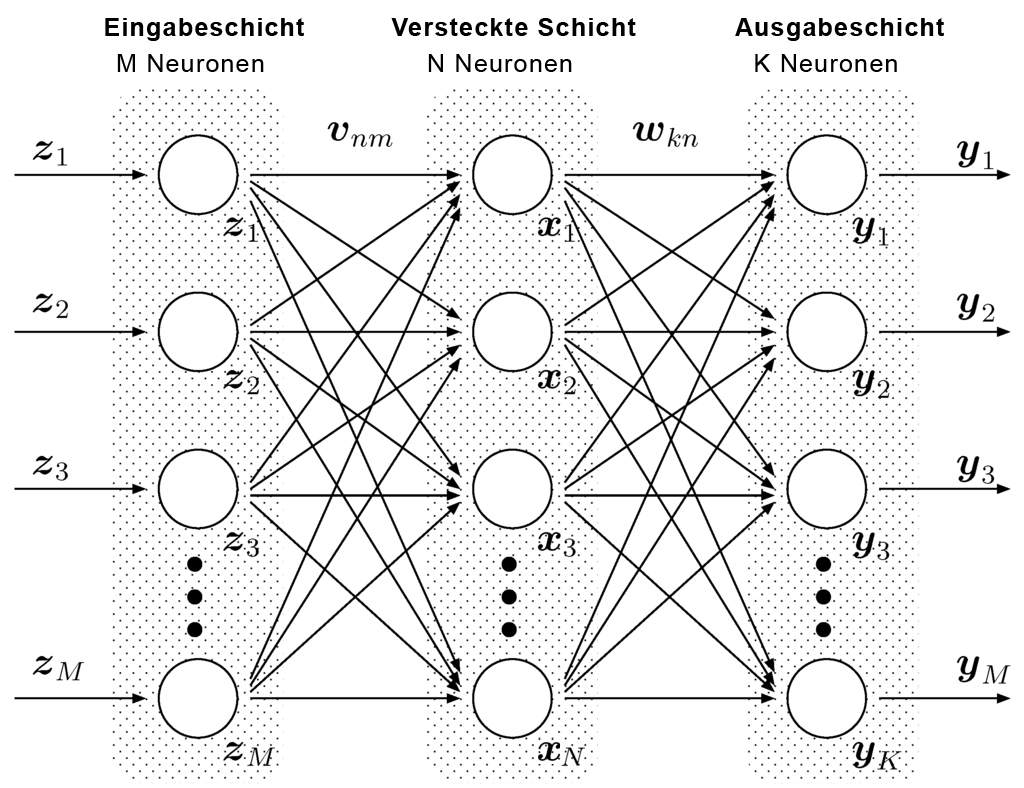
\includegraphics[width=\columnwidth]{Bilder/structure-mlp.jpg}
	\caption{Prinzipieller Aufbau MLP nach~\cite{MDPI}.}
	\label{fig:MLP}
\end{figure}
Am häufigsten kommen sogenannte \textit{Multilayer Perceptrons}~(MLP)~\cite{NNBraun}\cite{NNNauck}\cite{NNStanley} zum Einsatz. Ein generalisierter Aufbau ist beispielhaft in Abbildung~\ref{fig:MLP} zu sehen. Dieses MLP besteht aus einer Eingabe- und Ausgabeschicht mit $M$ bzw. $K$ Neuronen und einer versteckten Schicht mit $N$ Neuronen. Es handelt sich um ein vorwärtsgekoppeltes Modell, bei welchem jedes Neuron einer Schicht mit jedem Neuron der darauffolgenden Schicht verbunden ist. Dies nennt man volle Verbindung. \\
Die Eingangsschicht dient zum Verteilen der Daten $z_m$ mit $m=1,...,M$. Die Ausgabe eines jeden Neurons in der versteckten Schicht, dargestellt durch $x_n$ mit $n=1,...,N$, lässt sich durch Formel~\ref{eq:AusgabeVerdeckteSchicht} berechnen. Hierbei steht $v_{nm}$ für die jeweilige Gewichtung der Verbindungen zwischen den Neuronen der Eingabe- und der versteckten Schicht und $f$ für die Aktivierungfunktion~\cite{NNStanley}\cite{NNHaykin} des jeweiligen Neurons. 
\footnotesize
\begin{equation} 
x_n = f~(\sum_{m=1}^M v_{nm}z_m)
	\label{eq:AusgabeVerdeckteSchicht}
\end{equation}
\small
Die Ausgangswerte $y_k$, mit $k=1,...,K$, lassen sich äquivalent unter Hereinnahme der Werte $x_n$ und der Gewichte $w_{kn}$, sowie einer Aktivierungsfunktion $g$ berechnen, und gelten als Vertrauenswerte. Sie müssen gemäß der Aufgabenstellung interpretiert werden. 


\SubSection{Faltungsnetze} \label{sec:Faltungsnetze}
\todo[inline, color=yellow]{Laura} 
Im Folgenden wird genauer auf CNNs eingegangen, da diese die Grundlage, für die meisten der in den folgenden Kapitel vorgestellten Ansätze, bilden. Vereinfacht ausgedrückt besteht ein CNN aus einer Vernetzung von Faltungsoperationen mit unterschiedlichen Filtermasken. CNNs kommen, bedingt durch ihre Architektur, oft zum Einsatz, wenn große Datenmengen von einem NN verarbeitet werden sollen. Ein schematischer Aufbau ist in Abbildung~\ref{fig:CNN} zu sehen. \\
\begin{figure}
	\flushleft
	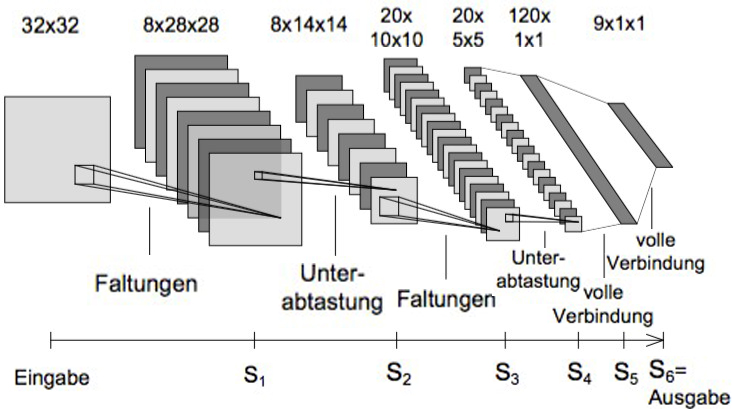
\includegraphics[width=\columnwidth]{Bilder/structure-cnn.jpg}
	\caption{Prinzipieller Aufbau Faltungsnetz nach~\cite{Osadchy}.}
	\label{fig:CNN}
\end{figure}
Jedes Pixel eines Feldes, das auf der Abbildung zu sehen ist, wird durch ein Neuron repräsentiert. Die Felder sind in Schichten organisiert. Die Eingangsschicht fungiert, vergleichbar mit den MLPs aus Kapitel~\ref{sec:NeuronaleNetze}, als Verteiler der Information an die Neuronen der nächsten Schicht $S_1$. Die Besonderheit eines CNNs sind die sich abwechselnd durchgeführte Faltung und anschließende Unterabtastung. Zwischen den Schichten $S_4$ und $S_6$ ähnelt das Modell einem MLP, da die Neuronen schichtweise voll verbunden sind.\\
Im Allgemeinen wird für eine Faltung eine Filtermaske $h$, also ein endlicher, zweidimensionaler Koeffizientensatz, wie in Formel~\ref{eq:Filtermaske} zu sehen, verwendet. Hierbei stehen $x$ und $y$ jeweils für die horizontale bzw. die senkrechte Bildkoordinate. Die Anzahl der Koeffizienten $a_{xy}$, wird in der Horizontalen mit $N_{hx}$ und im Vertikalen mit $N_{hy}$ bezeichnet. 
\footnotesize
\begin{equation} 
	h(x,y) = \left\lbrace
  \begin{array}{l@{}l}
   0~f\ddot{u}r~x<-\lfloor\frac{N_{hx}-1}{2}\rfloor~\vee~y<-\lfloor\frac{N_{hy}-1}{2}\rfloor\\
    0~f\ddot{u}r~x>\lfloor\frac{N_{hx}-1}{2}\rfloor~~~~\vee~y>\lfloor\frac{N_{hy}-1}{2}\rfloor \\
    a_{xy}
  \end{array}
  \right.	
	\label{eq:Filtermaske}
\end{equation}
\small  
Formel~\ref{eq:Faltung} beschreibt die Faltung eines Eingangssignals $s$ mit einer Filtermaske $h$, wobei I das Ausgangssignal in Abhängigkeit von $x$ und $y$ beschreibt.
\footnotesize
\begin{equation}
\begin{aligned}
I(x,y) = (s*h)(x,y) = \\
\sum_{m_x=-\infty}^\infty \sum_{m_y=-\infty}^\infty s(m_x,m_y) \cdot h(x-m_x,y-m_y) 
\end{aligned}
	\label{eq:Faltung}
\end{equation}
\small
Im Fall eines CNNs wird die Faltung, die wie in Abbildung~\ref{fig:CNN} zu sehen, beispielsweise zwischen der Eingangsschicht und $S_1$ vollzogen wird, durch die Verbindung zwischen den Neuronen zweier Felder modelliert. Dabei entsprechen die Gewichte der Neuronen genau den Filterkoeffizienten $a_{xy}$. Für ein jedes Feld sind diese Koeffizienten konstant, was bedeutet, dass alle Neuronen eines Feldes mit nur einem Gewicht auskommen. Dieses Prinzip nennt man geteilte Gewichte. \\
Im CNN wird nach jeder Faltung eine Unterabtastung durchgeführt um zu gewährleisten, dass die Dimension der Eingangsdaten schrittweise an die Dimension des Ausgangsvektors angepasst wird. Hierzu wird meist eine bilineare Unterabtastung um den Faktor 2 vorgenommen. Allgemeiner betrachtet werden $n$x$n$ Werte zu einem Wert zusammengefasst.\\
Wie zu Beginn des Kapitels erwähnt, haben CNNs gegenüber den MLPs den Vorteil, dass sie nahezu beliebig hochskaliert werden können und somit gut geeignet für große Datenmengen sind. Dies liegt vor allem daran, dass die Neuronen nur lokal verbunden sind und sich somit das Prinzip der geteilten Gewichte zu Nutze gemacht werden kann. Ein weiterer Vorteil von CNNs, der vor allem in der Bildverarbeitung genutzt wird, ist das sie translationsinvariant sind.

\SubSection{Training Faltungsnetze} \label{sec:Training}
\todo[inline, color=yellow]{Laura} 
Meistens werden CNNs mittels der \textit{back-propagation} Methode trainiert. Bei dieser überwachten Lernmethode bedarf es einer großen Menge an vorher klassifizierten Eingabematerialien~\cite{5537907}. \\
In den Faltungsschichten kann der Fehler der vorangegangen Schicht nach Formel \ref{eq:Training} berechnet werden. Dabei steht $E$ für den Fehler in der jeweiligen Schicht $l$ gemacht wird. Während $x^l$ für die Eingabe in die Schicht steht, bezeichnet $y^l$ die Ausgabe der entsprechenden Schicht. Die Größe der Eingabe wird der Einfachheit halber als quadratisch, also $mxm$-groß angenommen. Die Gewichtung wird mit $w$ bezeichnet. Um die Formel in der Realität anzuwenden, muss die linke und obere Grenze de Eingabeinhaltes, z.B. eines Bildes, mit Nullen ergänzt werden. Ansonsten wäre es nicht möglich den Fehler für Pixel zu berechnen, welche näher als $m$ an den entsprechenden Rändern liegen. \\
\footnotesize
\begin{equation}
\begin{aligned}
\frac{\delta E}{\delta y_{ij}^{l-1}} = \sum_{a=0}^{m-1} \sum_{b=0}^{m-1} \frac{\delta E}{\delta x_{(i-a)(j-b)}^{l}} \frac{\delta x_{(i-a)(j-b)}^{l}}{\delta y_{ij}^{l-1}}  \\
= \sum \limits_{a=0}^{m-1} \sum \limits_{b=0}^{m-1} \frac{\delta E}{\delta x_{(i-a)(j-b)}^{l}} w_{ab}
\end{aligned}
	\label{eq:Training}
\end{equation}
\small
Die Schichten, in denen die Unterabtastung stattfindet, leisten kaum Beitrag zum eigentlichen Lernprozess des CNNs. Hier wird das Problem allerdings reduziert, da $n$x$n$ Werte in einem einzigen resultieren. \\
Weil alle Gewichtungen $w$ mittels des \textit{back-propagation} Algorithmus während des Trainings angepasst werden, können CNNs laut LeCun als Erzeuger ihrer eigenen Merkmalextraktion gesehen werden \cite{LeCun:1998:CNI:303568.303704}.








\Section{Konzeption} \label{sec:Konzeption}
\todo[inline, color=yellow]{Vera} 
Vor der eigentlichen Videoproduktion muss das Vorhaben zunächst konzipiert und detailliert geplant werden. Dies bezieht sich vor allem auf die kreativen Prozesse des Drehbuchschreibens und darauffolgend die gesamte Projektplanung und -vorbereitung. Naturgemäß sind NN weniger sinnvoll für die Planung von Projekten. Doch in den letzten Jahren wurde damit begonnen zu erforschen, ob sich mit Hilfe von NN kreative Prozesse umsetzen lassen und sie eine eigene Kreativität entwickeln können. In diesem Sinne ist Kreativität auch mit sinnvollen selbstständigem Denken oder Entscheiden gleichzusetzen, was  im Entstehungsprozess von Drehbüchern unumgänglich ist.

\SubSection{Aktueller Stand} \label{sec:SOTAVorverarbeitung}
\todo[inline, color=yellow]{Vera} 
Es gibt bereits erste Versuche mit Hilfe von NN automatisch sinnvolle Texte oder Dialoge zu erstellen, die auf bekannten Texten und Storylines basieren.

\Section{Produktion} \label{sec:Produktion}
\todo[inline, color=red]{Laura} 
\textcolor{red}{muss angepasst werden} \\
In diesem Kapitel werden zunächst Ansätze vorgestellt, die auf Grundlage von NNs Arbeitsschritte bei der Produktion von Videos übernehmen bzw. vereinfachen könnten (vgl. Kapitel~\ref{sec:SOTAProduktion}). Dazu ist an zu merken, dass diese Ansätze meist in einem anderen Kontext entwickelt wurden und ggf. eine Anpassung an die Standards einer Produktion stattfinden müsste. \\

In Kapitel~\ref{sec:Vondrick} wird ein Ansatz zur automatisierten Generierung von Szenendynamiken in Hinsicht auf Funktionsweise und Arbeitserleichterung für die Videoproduktion analysiert. 


\SubSection{Aktueller Stand Musikgenerierung} \label{sec:SOTAProduktion}
\todo[inline, color=yellow]{Laura} 
Es gibt verschiedene Ansätze NNs zu nutzen, um Musik automatisiert generieren zu lassen. Im Folgenden werden drei Ansätze kurz vorgestellt, welche alle rückgekoppelte Neuronale Netze (RNN) benutzen. \\
An der \textit{University of Washington} ist im Rahmen einer Projektarbeit ein Musik Generator namens \textit{Algo Rythm} entstanden~\cite{Algorithm}. Für die Umsetzung habend die Studierenden um Timmerman RNNs geeignet trainiert. Der Quellcode kann auf Github \cite{AlgorithmGit} eingesehen werden.\\
Ein weiterer Ansatz, der in \cite{eck+lapalme:2008} beschrieben wird, arbeitet ebenfalls mit einem RNN, welches mit einem Autokorrelation-basierte Prädiktor kombiniert wird. Dabei soll die Struktur von Musikstücken erlernt werden, indem zunächst die folgende Note einer Tonreihenfolge vorausgesagt werden soll. \\
Der letzte Ansatz benutzt ebenfalls RNNs um auf Grundlage einer Notensequenz eine Musikstück zu komponieren \cite{browne2001system}. Dabei wird die Eingabesequenz zunächst interpretiert. Anschließend sorgen zwei RNN basierte Algorithmen für die Produktion von sowohl Rhythmus, als auch die Vorhersage der nächsten Note. \\

Alle drei Ansätze weisen hohes Potential auf, wenn es darum geht Musikstücke automatisiert zu generieren. Über das Genre des zugeführten Musikmaterials lässt sich die gewünschte Ausgabe begrenzt steuern. Es wäre durchaus vorstellbar, so Musik für eine Filmproduktion zu generieren.






\SubSection{Szenendynamik nach Vondrick et al.} \label{sec:Vondrick}
\todo[inline, color=red]{Laura} 
Mit dem Ansatz von Vondrick et al.~\cite{VondrickPT16} können aus Einzelbildern ganze Szenen Dynamiken erstellt werden, welche zum einen für die Klassifizierung und zum anderen für die Vorhersage von Bewegung genutzt werden kann. Das Resultat sind kleine Videos mit einer Auflösung von 65x64 Pixeln und 32 Einzelbildern. \\
Die Grundlage für dieses Verfahren bilden zwei CNNs, die als \textit{Generative Adversarial Networks} (GAN) \cite{NIPS2014_5423} fungieren. Die beiden Netze können als Gegenspieler angesehen werden. Während der Generator $G$ für die Generierung von einer Videosequenz auf Grundlage eines Standbildes zuständig ist, soll der Diskriminator $D$ zwischen den so erzeugten Videos und realen Videosequenzen differenzieren können. Um dies zu erreichen werden beide GANs, wie in Formel 1 des Papers~\cite{VondrickPT16} zu sehen gegeneinander trainiert. Das Minimierungs- bzw. Maximierungsproblem wird hierzu mittels Gradientenverfahren gelöst. \\
Das Training der beiden Netze erfolgt unüberwacht. Da sich ähnliche Objekte in der Regel auch ähnliche Bewegungsmuster aufweisen, lassen die Autoren das zur Verfügung stehende Videomaterial in Kategorien (Strand, Babys, Golf und Züge) einteilen. Zudem sorgt ein Stabilisierungsalgorithmus dafür, dass bei dem gesamten Testmaterial von einer statischen Kamera ausgegangen werden kann und die zu erlernende Szenendynamik nicht durch eine Bewegung der Kamera verfälscht wird. Für jede dieser Kategorien wird dann ein eigenes Pärchen bestehend aus Generator und Diskriminator trainiert. \\
Bevor die beiden CNNs $G$ und $D$ auf die beschriebene Art trainiert werden können, müssen sie erst einmal ihren Aufgaben entsprechend aufgebaut werden. \\
\begin{figure}
	\flushleft
	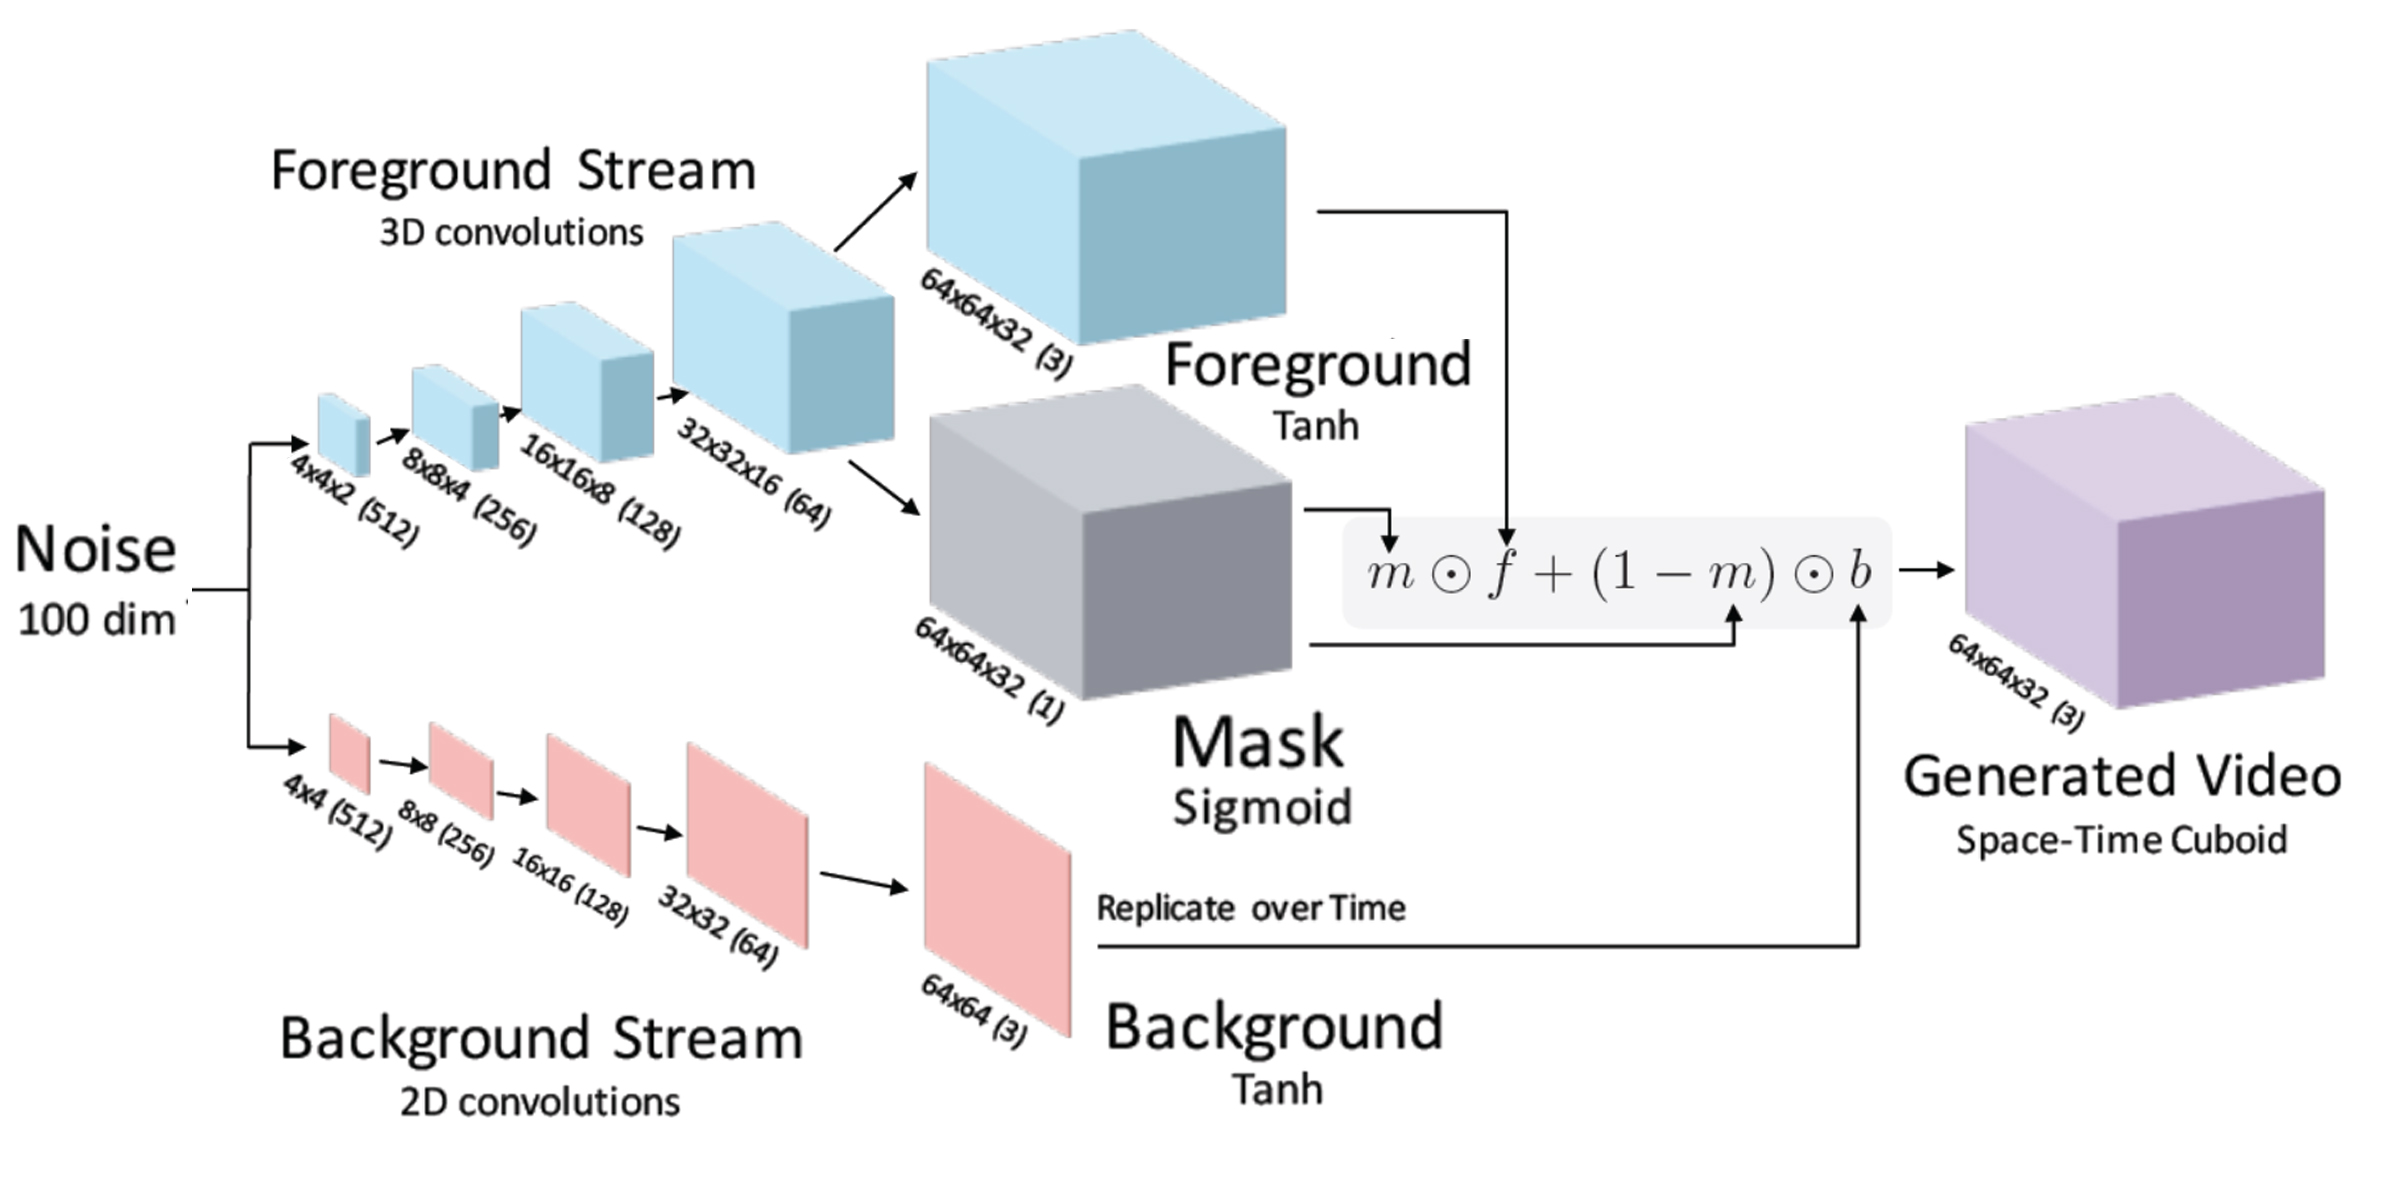
\includegraphics[width=\columnwidth]{Bilder/generator2.jpg}
	\caption{Aufbau Generator nach~\cite{VondrickPT16}.}
	\label{fig:generator}
\end{figure}
Den Aufbau des Generators, welchen Vondrick et al. genutzt haben, sieht man in Abbildung~\ref{fig:generator}. Im Gegensatz zu dem in Kapitel~\ref{sec:Faltungsnetze} beschriebenen, gewöhnlichen CNN, wird hierbei keine Unterabtastung vorgenommen, sondern die Menge der Daten von Schicht zu Schicht erweitert. Zudem werden die Eingabedaten für die Verarbeitung in zwei Datenströme aufgeteilt. Während in dem eine Strom der statische Hintergrund entsprechend vergrößert wird, wird in dem anderen die Bewegung des sich im Vordergrund befindlichen Objektes vorhergesagt. Beide Teile werden dann am Ausgang nach Formel~\ref{eq:Generator} zusammengefasst.
\footnotesize
\begin{equation}
\begin{aligned}
G(z) = m(z) \odot f(z) + (1-m(z))\odot b(z)
\end{aligned}
	\label{eq:Generator}
\end{equation}
\small
Dafür ist die binäre Maske $m$ so gewählt, dass sie überall den Wert eins hat, wo der Vordergrund übernommen werden soll und ansonsten nur Nullen enthält. \\
Der Diskriminator hat einen wesentlich simpleren Aufbau, der in Abbildung~\ref{fig:discriminator} zu sehen ist. Dabei muss die Eingabeschicht eben so groß sein, wie die Ausgabeschicht des Generators.\\
\begin{figure}
	\flushleft
	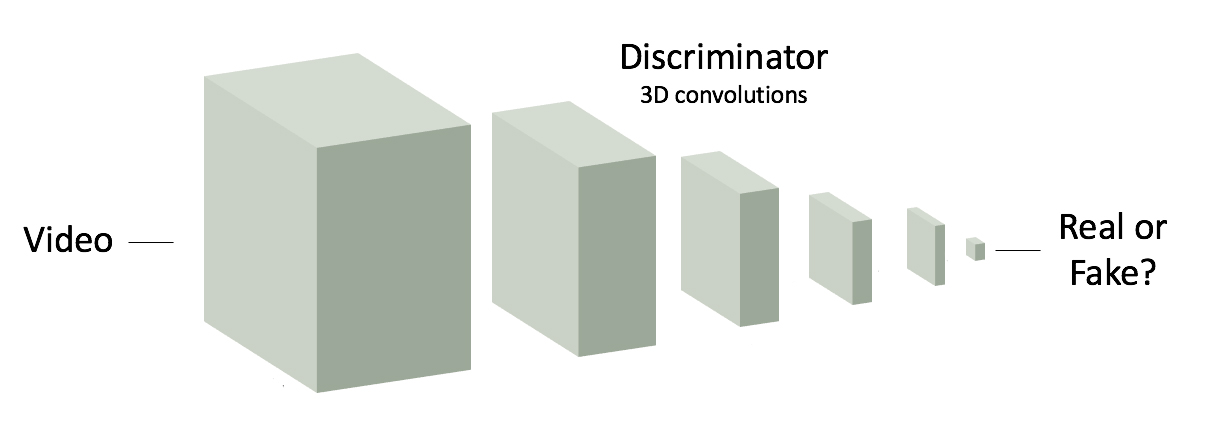
\includegraphics[width=\columnwidth]{Bilder/discriminator.jpg}
	\caption{Aufbau Diskriminator nach~\cite{VondrickPT16}.}
	\label{fig:discriminator}
\end{figure}
Die Bedeutung für so erzeugte Bewegtbildsequenzen für die Automatisierung der Produktion von Filmen, wird im nächsten Kapitel diskutiert.






\SubSection{Bewertung des Ansatzes von Vondrick} \label{sec:VondrickConclusion}
\todo[inline, color=red]{Laura} 
Das in Kapitel~\ref{sec:Vondrick} beschriebene Verfahren schafft es automatisiert aus einem Einzelbild eine kurze und niedrig aufgelöste Bewegtbildsequenz zu erstellen. Hierbei wir vor allem die Szenendynamik in den meisten Fällen annähernd realistisch vorhergesagt, wobei die Modellierung des sich bewegenden Bildinhaltes eher mangelhaft ist. Trotz des hohen Bedarfs an Trainingsmaterial und den damit verbundenen Zeitaufwand, kann das System ohne menschliche Hilfe eigenständig Kategorisieren, Trainieren und letztendlich Szenendynamiken generieren. Gegen einen Einsatz in der Videoproduktion sprechen die geringe Auflösung und Zeitspanne die bisher abgedeckt werden kann. Zudem kann in einer Szene nicht immer nur von einem sich bewegenden Objekt ausgegangen werden. Und ein trainieren von Netzen für alle denkbaren Kategorien ist sehr aufwendig. Dennoch könnte der Ansatz als Grundlage für einen ausgereifteren Algorithmus dienen, der beispielsweise die Anweisungen des Drehbuchs mit einbezieht und somit eine Generierung von planbareren Szenen ermöglicht. \\
Der jetzige Stand des Algorithmus könnte beispielsweise für die Generierung von GIFs oder Simulationen genutzt werden. Zudem könnte der Ansatz, mit etwas Anpassung, anstatt Szenendynamiken in Form von Videos darzustellen, Bewegungsvektoren aus einem Standbild vorhersagen und somit in der Videocodierung Einsatz finden. 




\Section{Postproduktion} \label{sec:Postroduktion}
\todo[inline, color=red]{Vera} 
\SubSection{Aktueller Stand} \label{sec:SOTAPostproduktion}
\todo[inline, color=red]{Vera} 

\Section{Zusammenfassung} \label{Zusammenfassung}
\todo[inline, color=red]{Vera} 




\Urlmuskip=0mu plus 1mu\relax %Bricht Link in Bibfile um
\bibliographystyle{latex8} 
\bibliography{psm}

\end{document}

